\PassOptionsToPackage{dvipsnames}{xcolor}
\documentclass[mathserif]{beamer}
\usetheme{Malmoe}
%\usecolortheme{beaver}
\useoutertheme{infolines}
\setbeamercolor{frametitle}{fg=BlueViolet,bg=gray!10}
\setbeamercolor{section in head/foot}{bg=black, fg=white}
\setbeamercolor{author in head/foot}{bg=BlueViolet, fg=white}
\setbeamercolor{title in head/foot}{bg=black,fg=white}
\setbeamercolor{date in head/foot}{bg=BlueViolet,fg=white}
\setbeamercolor{frametitle}{bg=BlueViolet!10,fg=BlueViolet}
\setbeamercolor{normal text}{bg=black,fg=black}
\setbeamercolor{structure}{bg=BlueViolet!10, fg=BlueViolet}
\setbeamercolor{title}{bg=BlueViolet!10,fg=BlueViolet}
\setbeamercolor{titlelike}{bg=BlueViolet!10,fg=BlueViolet}
\setbeamercolor{background canvas}{bg=white}
\setbeamercolor{block body}{bg=BlueViolet!10, fg=black}
\setbeamertemplate{blocks}[rounded][shadow=false]
\usepackage{animate}
\usepackage{multicol}
\usepackage[utf8]{inputenc}
\usepackage[english,spanish]{babel}
\usepackage{amsmath}
\usepackage{amsfonts}
\usepackage{amssymb}
\usepackage{tikz}
\usepackage{braket}
\usepackage{listings}
\usepackage{textpos}
%\usepackage[absolute,overlay]{textpos}
\lstset{basicstyle=\ttfamily,
  showstringspaces=false,
  commentstyle=\color{blue},
  keywordstyle=\color{violet},
%  numbers=left
}
\setbeamertemplate{theorem}[ams style]
\setbeamertemplate{theorems}[numbered]
\usepackage{verbatim}
\usepackage{xcolor}
\usepackage{alltt}
\usetikzlibrary{mindmap, trees}
\usepackage{graphicx}
\author[Daniel C. Padilla-González]{Daniel C. Padilla-González$^{1,2}$}
\title{Supervised Learning of Ising Model\\ Part I}
\vspace*{0.6cm}
\titlegraphic{
\begin{flushright}
%
\includegraphics[height=1.2cm]{Logo1.jpg}\hspace*{.2cm}~%

\includegraphics[height=1.2cm]{Logo1.png}\hspace*{0.1cm}
\end{flushright}
}
\institute[]{$^{1}$Universidad Nacional de Colombia\\$^{2}$E-mail: \texttt{dcpadillag@unal.edu.co} }
 
\date{02/03/2018} 
%\subject{} 
%\newcommand{•}{•}
\newcommand{\code}[1]{\texttt{\textcolor{violet}{#1}}}
\newtheorem{defin}{Definition }
\setbeamertemplate{defin}[numbered]
\setbeamertemplate{caption}[numbered]

\begin{document}
\renewcommand{\figurename}{Figure}
\renewcommand{\tablename}{Table}
\newcommand{\pa}[2]{\frac{\partial #1}{\partial #2}}
\begin{frame}
\maketitle
\end{frame}

\addtobeamertemplate{frametitle}{}{%
\begin{textblock*}{0mm}(.95\textwidth,-0.96cm)

\includegraphics[height=.9cm]{Logo1.png}
\end{textblock*}}

%\begin{frame}
%\tableofcontents
%\end{frame}

\begin{frame}
\begin{multicols}{2}
\tableofcontents
\end{multicols}
\end{frame}


\section{What is Machine Learning?}
\begin{frame}{Machine Learning Phases of Matter}
\begin{figure}[H]
\centering
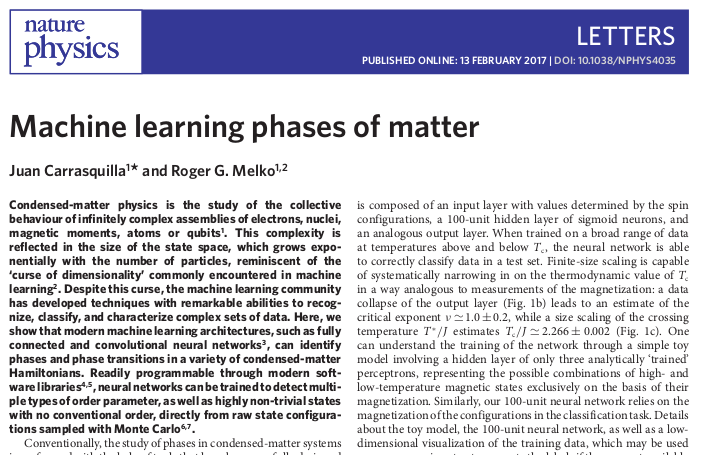
\includegraphics[scale=0.4]{figures/carrasquilla.png}
\end{figure}
\end{frame}

\begin{frame}{What is Machine Learning?}
\begin{multicols}{2}
\small Machine Learning refers to some kind of algorithms which help  a computer to learn.

\begin{figure}[H]
\centering
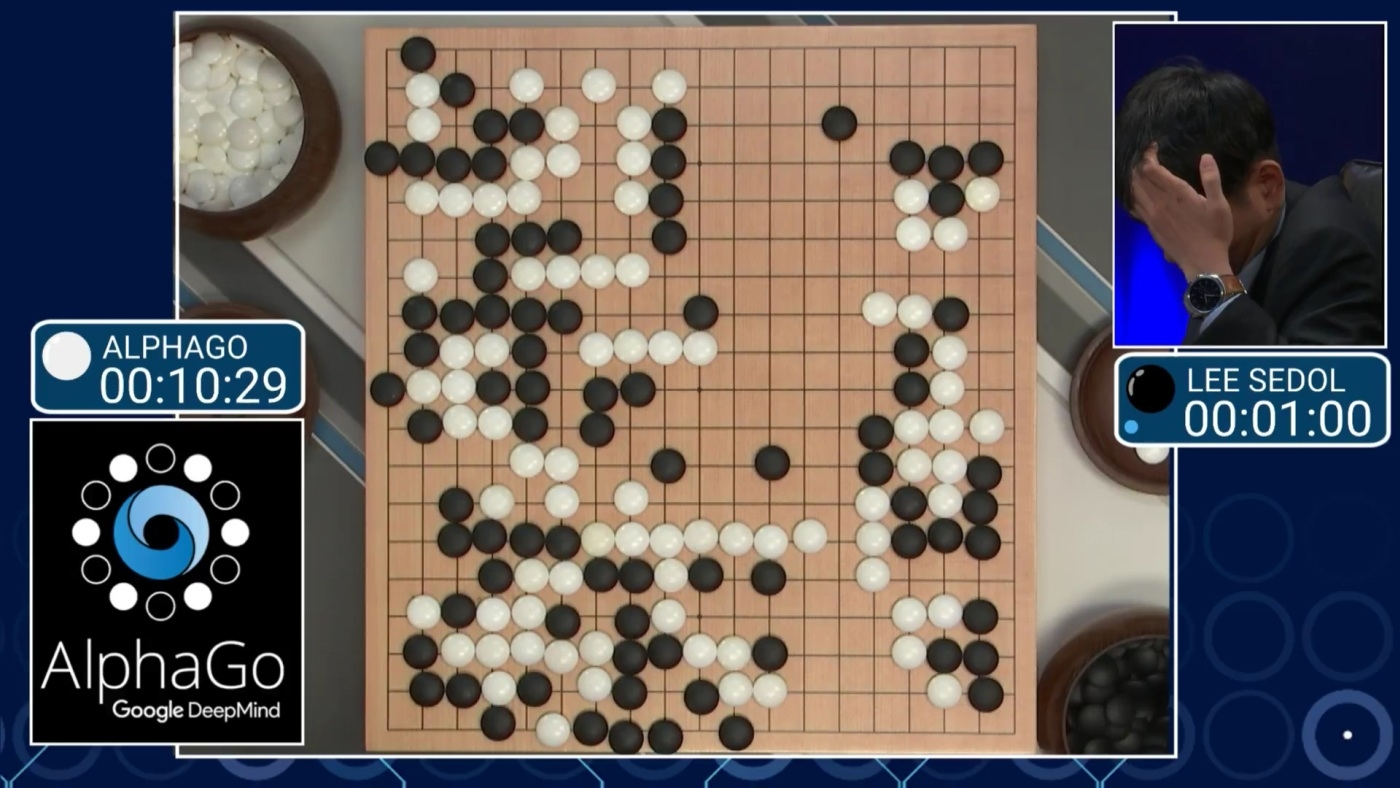
\includegraphics[scale=0.15]{figures/alphaGO.jpeg}
\end{figure}

\columnbreak

\begin{figure}[H]
\centering
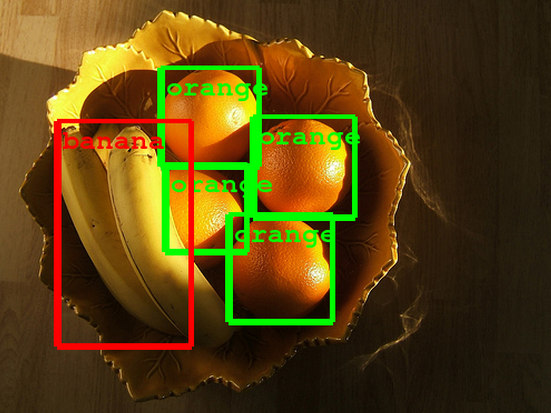
\includegraphics[scale=0.2]{figures/rimages.jpg}
\end{figure}

\end{multicols}
\end{frame}


\subsection{Learning Tasks}
\begin{frame}{Learning Tasks}
\begin{multicols}{2}
\begin{figure}[H]
\centering
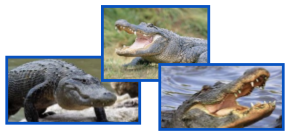
\includegraphics[scale=0.5]{figures/supervised_1.png}
\end{figure}

\begin{figure}[H]
\centering
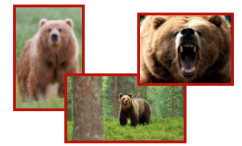
\includegraphics[scale=0.5]{figures/supervised_2.png}
\end{figure}

\columnbreak
\begin{itemize}
\item Supervised learning (labeled data)
\item Unsupervised learning (unlabeled data)
\item Reinforcement learning ('reward' data)
\end{itemize}
\end{multicols}
\end{frame}


\subsection{Supervised Learning}
\begin{frame}{Supervised Learning}
\begin{multicols}{2}
\small There is several models for a supervised learning

\begin{enumerate}
\item The linear model ($f(x)=wx+b$)
\item Kernel learning ($f(x)=w\Phi(x)$)
\item Neural Networks ($f(x)=\sigma(wx+b)$)
\end{enumerate}
\columnbreak
\begin{figure}[H]
\centering
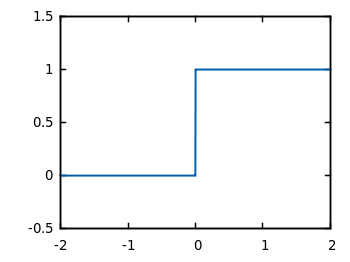
\includegraphics[scale=0.4]{figures/step.png}
\end{figure}

\end{multicols}
\end{frame}



\section{Neural Networks}
\begin{frame}{Neural Networks}
\begin{figure}[H]
\centering
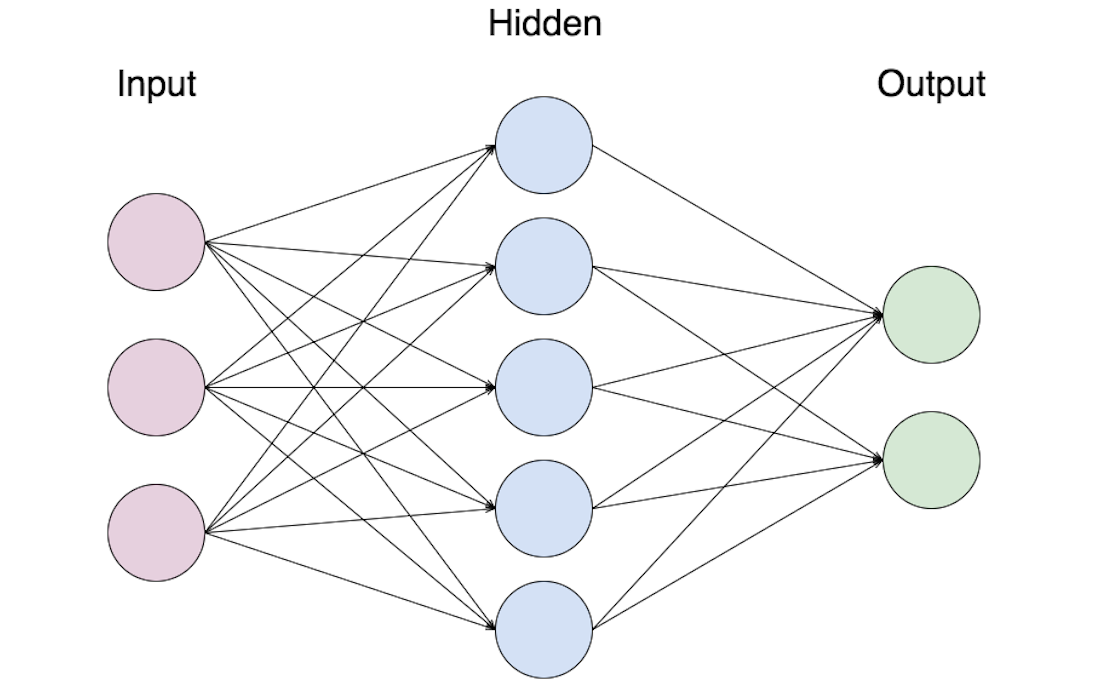
\includegraphics[scale=0.3]{figures/nnetwok.png}
\end{figure}
\end{frame}


\subsection{Hidden Layers}
\begin{frame}{Hidden Layers}
\begin{multicols}{2}
\begin{figure}[H]
\centering
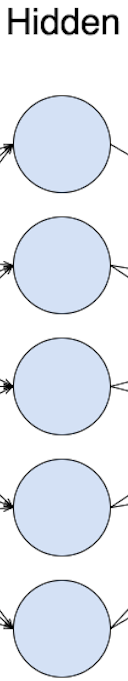
\includegraphics[scale=0.3]{figures/hlayer.png}
\end{figure}
\columnbreak

Each hidden layer contains a certain number of nodes called \textit{neurons} which transmit information from the input date.

\begin{align*}
z=&f(x)=\sigma(wx+b)\\
\sigma(x)=&\frac{1}{1+e^{-x}}.
\end{align*}

\end{multicols}
\end{frame}

\begin{frame}{Learning}
\small Given an initial prediction for the input data (1 or 0 depending if the activation of a neuron $z$ overcome some threshold or not) the machine is trained to get an accurate prediction

\begin{equation*}
cost=\frac{1}{N}\sum_{j}{(f(x_{j})-y_{j})^{2}}
\end{equation*}

The idea is minimized the cost function and set

\begin{align*}
w&=w-\nabla_{w}cost\\
b&=b-\nabla_{b}cost
\end{align*}
\end{frame}

\subsection{Example: The Flower Problem}
\begin{frame}{Example: The Flower Problem}
\begin{table}
\centering
\begin{tabular}{|c|c|c|c|c|c|c|c|c|c|}
\hline
Color & Red & Blue & Red & Blue & Red & Blue & Red & Blue & ?\\\hline
Length & 3.0 & 2.0 & 4.0 & 3.0 & 3.5 & 2.0 & 5.5 & 1.0 & 1.5\\\hline
Width & 1.5 & 1.0 & 1.5 & 1.0 & 0.5 & 0.5 & 1.0 & 1.0 & 1.5 \\\hline
\end{tabular}
\end{table}

\begin{figure}[H]
\centering
\begin{tabular}{cc}
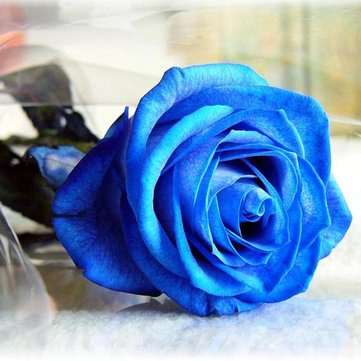
\includegraphics[scale=0.3]{figures/brose.jpg} &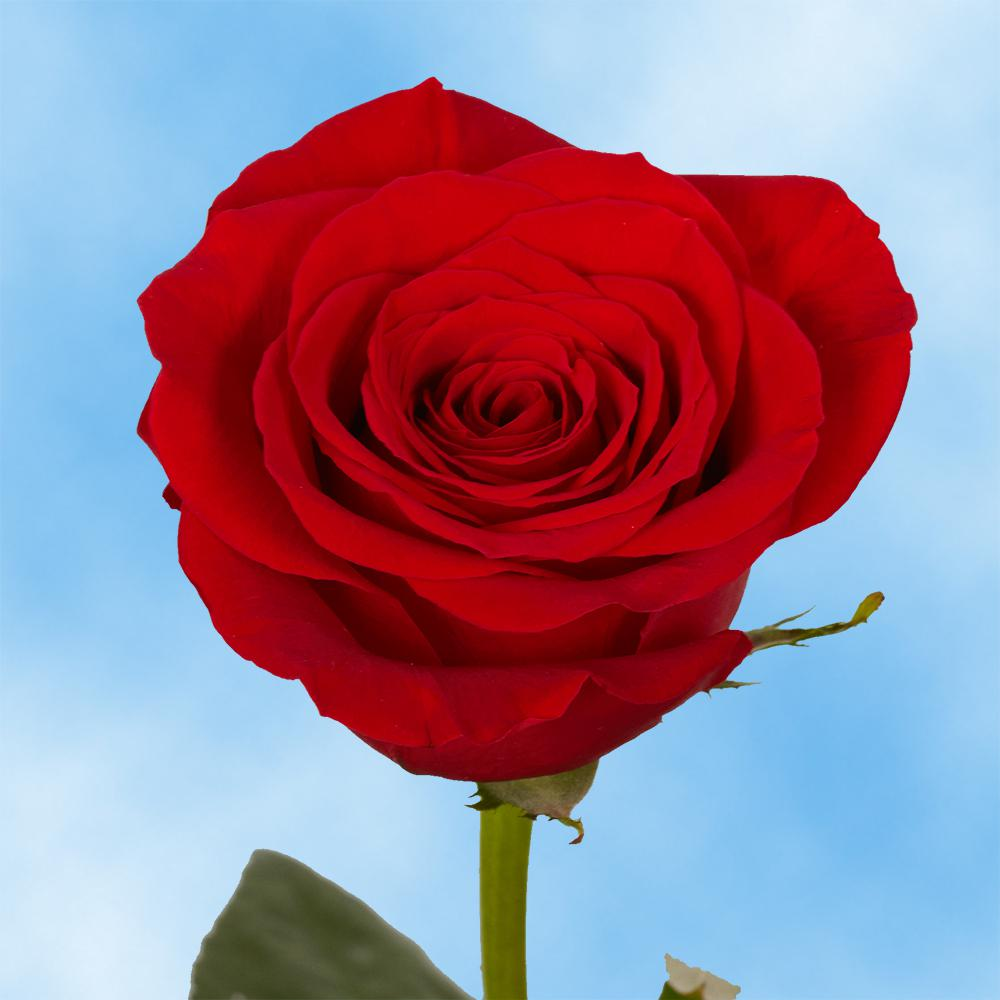
\includegraphics[scale=0.1]{figures/rrose.jpg}
\end{tabular}
\end{figure}
\end{frame}

\section{Supervised Learning of Ising Model}
\begin{frame}{Supervised Learning of Ising Model}

\begin{figure}[H]
\centering

\includegraphics[scale=0.4]{figures/wessel.png}
\end{figure}
\end{frame}

\subsection{Input data -Monte Carlo Cluster Algorithm-}
\begin{frame}{Input data -Monte Carlo Cluster Algorithm-}

\end{frame}

\subsection{Hidden Layer}
\begin{frame}{Hidden Layer}

\end{frame}

\subsection{Output Layer}
\begin{frame}{Output Layer}

\end{frame}

\subsection{Results}
\begin{frame}{Results}

\end{frame}
\end{document}


